%
% Tesi D.S.I. - modello preso da
% Stanford University PhD thesis style -- modifications to the report style
%
%%%%%%%%%%%%%%%%%%%%%%%%%%%%%%%%%%%%%%%%%%%%%%%%%%%%%%%%%%%%%%%%%%%%%%%%%%%
%                                                                         %
%			TESI DOTTORATO                                                   %
%			______________                                                   %
%                                                                         %
%			AUTORE: Elena Pagani                                             %
%                                                                         %
%			Ultima revisione: 7.X.1998                                       %
%                                                                         %
%%%%%%%%%%%%%%%%%%%%%%%%%%%%%%%%%%%%%%%%%%%%%%%%%%%%%%%%%%%%%%%%%%%%%%%%%%%
%
%
\documentclass[12pt]{report}
   %\renewcommand{\baselinestretch}{1.5}      % interline spacing
%
% \includeonly{}
%
%			PREAMBOLO
%

\usepackage[a4paper]{geometry}
\usepackage{amssymb,amsmath,amsthm}
\usepackage{graphicx}
\usepackage{bm}
\usepackage{url}
\usepackage{hyperref}
\usepackage{epsfig}
\usepackage[italian]{babel}
\usepackage{setspace}
\usepackage{tesi}
\usepackage{biblatex}
\usepackage{algorithm}% http://ctan.org/pkg/algorithms
\usepackage{algpseudocode}%
\usepackage[detect-all]{siunitx} 
\makeatletter
\renewcommand{\ALG@name}{Algoritmo}
\makeatother

% per le accentate
\usepackage[utf8]{inputenc}
%
\newtheorem{myteor}{Teorema}[section]
%
\theoremstyle{definition}
\newtheorem{exmp}{Esempio}[section]

%
\newenvironment{teor}{\begin{myteor}\sl}{\end{myteor}}
\bibliography{references.bib}

%
%
%			TITOLO
%
\begin{document}
\title{Rilevazione di fake news basata sull'induzione di insiemi fuzzy}
\author{Giovanni LAGANÀ}
\dept{Corso di Laurea Magistrale in Informatica}
\anno{2019-2020}
\matricola{928792}
\relatore{Prof. Dario MALCHIODI}
\correlatore{Prof. Alfio FERRARA}
%
%        \submitdate{month year in which submitted to GPO}
%		- date LaTeX'd if omitted
%	\copyrightyear{year degree conferred (next year if submitted in Dec.)}
%		- year LaTeX'd (or next year, in December) if omitted
%	\copyrighttrue or \copyrightfalse
%		- produce or don't produce a copyright page (false by default)
%	\figurespagetrue or \figurespagefalse
%		- produce or don't produce a List of Figures page
%		  (false by default)
%	\tablespagetrue or \tablespagefalse
%		- produce or don't produce a List of Tables page
%		  (false by default)
%
%			DEDICA
%
\beforepreface
        {\hfill \Large {\sl \begin{flushright} Dedica da inserire.         
\end{flushright}         }}
%
%			PREFAZIONE
%
%\prefacesection{Prefazione}
%hkjafgyruet.
%
%%
%%
%%			ORGANIZZAZIONE
%\section*{Organizzazione della tesi}
%\label{organizzazione}
%La tesi \`e organizzata come segue:
%\begin{itemize}
%\item nel Capitolo 1 ....
%\end{itemize}
%
\afterpreface

%
%
%			CAPITOLO 1: 

\chapter*{Introduzione}
\addcontentsline{toc}{chapter}{Introduzione} \markboth{Introduzione}{} 
\onehalfspacing

Prova per citare tutti i libri
\cite{1,2,3,4,5,6,7,8,9,10,11,12,13,14,15,16,17,18,19,20,21,22}


\chapter{Stato dell'arte}
\label{Capitolo 1}
\onehalfspacing

Il Capitolo che apre questo elaborato è inerente allo stato dell'arte. Esso si compone come segue: la Sezione \ref{fakenews} descrive il problema delle fake news, menzionando la disciplina del fact-checking; la Sezione \ref{nlp} riporta le tecniche di elaborazione del linguaggio naturale, tipicamente di pulizia del testo per la fase di preprocessing, di rielaborazione e di embedding per convertire tale testo in un dominio numerico.
La Sezione \ref{insiemifuzzy} presenta il concetto della logica fuzzy e fornisce una motivazione del perchè essa sia uno strumento adeguato per il problema delle fake news.
Infine, la Sezione \ref{induzione} porta alla luce i protagonisti dell'induzione su insiemi fuzzy: le funzioni di appartenenza, i diversi tipi di kernel e di fuzzificatore.

\section{Fake news} \label{fakenews}
L'avvento dei news media e social media ha portato a una proliferazione e a un consumo crescenti di notizie.
\\
In generale, la circolazione di notizie su questi canali ha fatto sì che aumentassero esponenzialmente le cosiddette \textit{fake news}.
\\
Per fake news si intendono quelle notizie i cui fatti riportati volutamente non corrispondono alla realtà.
\\
In questo senso, si evidenzia la necessità di riconoscere e combattere questo fenomeno con l'obiettivo di contrastare il fomentare dell'odio, un'arma che al giorno d'oggi può essere usata come carburante di diffamazione, lucro, terrorismo e xenofobia.
\\
Il problema di questo tipo di notizie è che possono mischiarsi con tutte le altre, portando il lettore a confondere un fatto realmente accaduto con uno volutamente modificato a proprio vantaggio per un secondo fine.

\subsection{Fact-checking} \label{factchecking}
In generale, aldilà di quale sia il secondo fine di chi diffonde fake news, il nemico numero uno del giornalismo è la disinformazione.
Per questo motivo un lavoro da sempre svolto da giornalisti, e non, è quello del \textit{fact-checking}: si tratta di una serie di attività mirate alla verifica accurata e puntuale delle fonti.
Secondo questo criterio, la verifica delle fonti avrebbe il vantaggio di validare i fatti, non lasciando spazio ad avvenimenti non confermati da fonti autorevoli.
\\
Questo approccio, però, presenta delle criticità, ad esempio l'assunzione che una fake news non abbia fonti: esistono notizie che, pur attenendosi alle fonti, possono esaltare aspetti apparentemente secondari o di dettaglio che, se esasperati, possono alterare la narrazione di un fatto, fino a sconvolgerla.
\\
Un altro aspetto è che non è così semplice stabilire con certezza quando una fonte sia autorevole e quando no; inoltre, è opinabile assumere a priori che una fonte considerata autorevole non commetta mai a sua volta errori di questo tipo.
\\
Uno dei problemi maggiori, oltre al fatto che la verifica della veridicità di una notizia richieda del tempo, è che la smentita non finisce mai per avere la stessa risonanza e visibilità della notizia falsa. Questo evidenzia l'esigenza di trovare un metodo per prevenire il problema, piuttosto che risolverlo a posteriori.
\\
La necessità di arginare questo fenomeno ha spinto i media, soprattutto tradizionali, a impegnarsi in un costante lavoro di fact checking, lungo, impegnativo e reso ancora più difficile dal fatto che spesso le varie realtà agiscono in maniera autonoma.
\\
Ci si chiede, quindi, se il progresso in ambito informatico possa contribuire ad arginare il problema in maniera efficace.
\\
In letteratura sono stati fatti vari studi \cite{5, 6, 8, 9, 10, 11} per la cosiddetta automazione del fact-checking; inoltre, in \cite{15, 16, 21} sono stati proposti approcci che, principalmente, si suddividono in \textit{content-based} e \textit{context-based}.
\\
Mentre il primo lavora sul contenuto testuale a livello sintattico, il secondo estrapola il contesto, lavorando a livello semantico.

\section{Elaborazione del linguaggio naturale} \label{nlp}
L'analisi lessicale fa parte dell'ampia branca dell'informatica che prende il nome di NLP, \textit{Natural Language Processing}, che tra le sue varie declinazioni, presenta degli interessanti strumenti per poter estrarre delle features a partire da dati testuali come le notizie.


\subsection{Tecniche di pulizia del testo} \label{clean}
Come nella stragrande maggioranza dei dataset, anche in quelli testuali è presente del rumore, sia a "basso livello" nel contenuto dell'informazione, sia ad "alto livello" nella forma dei dati che si sta utilizzando.
\\
Possono essere molte le motivazioni che portano un dataset a presentare errori, anomalie o rumore al suo interno: 
l'annotazione manuale e dunque la componente di errore umano da parte di chi crea il dataset, oppure la processazione automatica utilizzata per raccogliere osservazioni, anch'essa può produrre risultati imprevisti.
\\
Nel caso dei dati trattati in questo elaborato, inoltre, si ha a che fare con informazioni provenienti dal web, dunque esiste una maggior probabilità di incontrare, in questo contesto, informazioni di natura digitale ricavate da pagine HTML o, addirittura, influenzate dal tipo di codifica scelto per rappresentare caratteri speciali.
\\
In tal senso esistono numerose tecniche per gestire il rumore e, seguendo la distinzione fatta all'inizio di questa Sezione, è possibile elencare alcune di esse.
\\
\\
Ad \textit{alto livello} si gestisce la presenza di:
\begin{itemize}
    \item valori mancanti
    \item osservazioni duplicate
    \item osservazioni vuote
\end{itemize}

mentre a \textit{basso livello}, tipicamente, si riscontrano:
\begin{itemize}
    \item caratteri speciali
    \item URLs
    \item parole contenenti numeri (es: username)
    \item punteggiatura
\end{itemize}

e altri numerosi casi che potrebbero essere aggiunti a questo elenco.
\subsection{Tecniche per rielaborare il testo}
Esistono, inoltre, delle tecniche per riadattare il testo in una forma più conveniente per sua la successiva elaborazione da parte di modelli matematici.
\\
Vari studi nel campo dell'Information Retrieval \cite{22}, infatti, hanno dimostrato che tecniche come la lemmatizzazione, la rimozione delle cosiddette \textit{stop word} e lo stemming possono migliorare sensibilmente i risultati ottenuti da tali modelli.

\subsection{Tecniche di embedding} \label{embedding}
Tipicamente, i modelli matematici utilizzati per l'apprendimento utilizzano un input in forma numerica.
\\
In questo senso, le tecniche di embedding intervengono proprio per trasformare il dato testuale in dato numerico.
Concretamente, questo equivale a trovare una rappresentazione numerica del testo, estraendo delle features.
\\
Due famose tecniche di embedding sono Word2Vec e Doc2Vec, i cui nomi lasciano già presagire il tipo di lavoro che intendono fare.
\subsubsection{Word2Vec} \label{w2v}
Si tratta di un algoritmo che ha l'obiettivo di trasformare le parole in vettori numerici.
Un corpus è composto da documenti, e ogni documento è composto da parole; ciascuna di queste parole, tramite Word2Vec, viene trasformata in un vettore di lunghezza $k$, dove $k$ indica il numero di features. 
\\
Word2Vec si basa sull'utilizzo di reti neurali \cite{3} ed è principalmente implementato tramite due modelli:
\begin{enumerate}
    \item Skip-Gram
    \item CBOW (Continuous Bag of Words)
\end{enumerate}

Inoltre vale la pena menzionare tre varianti di criteri di addestramento applicabili (Softmax, Negative sampling, Hierarchical Softmax), con diverse implicazioni riguardo efficienza e onere computazionale.
\\
Per entrambe le architetture l'input è un corpus di documenti, le cui parole vengono distinte in \textit{token}; ciascun token viene codificato con una rappresentazione one-hot.
\\
Per differenziare le due soluzioni, è necessario introdurre il concetto di contesto, poichè Skip-Gram e CBOW, relativamente ad esso, lavorano in due direzioni speculari:
mentre la prima si pone l'obiettivo di predire le parole di contesto a partire dal token corrente, la seconda ha lo scopo di predire il token corrente da una finestra di parole di contesto.

\paragraph{Skip-Gram}
Si stabilisce una finestra di dimensione $m$ e si scorre ogni token andando a vedere i termini in prossimità, osservando quelli all'interno del raggio $m$.
\\
\begin{figure}[!h]
    \centering
    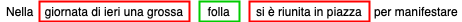
\includegraphics[scale = 0.7]{images/skip-gram.png}
    \caption{Esempio con finestra di contesto grande 5 token}
    \label{skipgram}
\end{figure}
\\
Per esempio se \textit{folla} è il token corrente, con $m = 5$ il confronto avviene con \{\textit{giornata}, \textit{di}, \textit{ieri}, \textit{una}, \textit{grossa}, \textit{si}, \textit{è}, \textit{riunita}, \textit{in}, \textit{piazza}\}.
\\
L'idea è cercare di costruire il mapping tra $X$, i token correnti (es: \textit{folla}), e $y$, i token estratti dalla finestra di contesto (es: \textit{piazza}).
\\
Seguendo la notazione tipica di un problema di apprendimento supervisionato, i token presi dalla finestra di contesto sono la variabile target da predire, apprendendo il tipo di relazione che sussiste tra  $X$ e $y$.
\\
Per farlo, come accennato in precedenza, si utilizza una rete neurale, passando la rappresentazione one-hot del dato a un'unità softmax (o le varianti sopracitate) per ottenere una distribuzione che indichi la probabilità che una specifica parola di contesto sia quella espressa dalla relativa componente.
\\
Infine, si utilizza il metodo del gradiente discendente per minimizzare una funzione di perdita, tipicamente l'entropia incrociata. 

\paragraph{CBOW}
Dualmente a Skip-Gram, CBOW si occupa di predire la parola centrale a partire dalla finestra di contesto.
\\
Dunque, riprendendo l'esempio precedente, si predice con quale probabilità si ottenga il token \textit{folla} a partire dalla finestra \{\textit{giornata}, \textit{di}, \textit{ieri}, \textit{una}, \textit{grossa}, \textit{si}, \textit{è}, \textit{riunita}, \textit{in}, \textit{piazza}\}.
\\
\begin{figure}[!h]
    \centering
    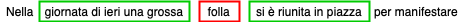
\includegraphics[scale = 0.7]{images/cbow.png}
    \caption{Esempio con finestra di contesto grande 5 token}
    \label{cbow}
\end{figure}
\\
Anche in questo caso vengono usati la rete neurale e il metodo del gradiente discendente per ottenere l'embedding.
\\
\\
In generale, per la natura di queste tecniche, per ottenere una rappresentazione compatta dell'intero documento, si rende necessario l'utilizzo in una seconda fase di una tecnica di aggregazione (es: media aritmetica, mediana, aggregazione del kernel di Fisher \cite{19}).

\subsubsection{Doc2Vec} \label{d2v}
Doc2Vec nasce come evoluzione di Word2Vec: in questo caso, anzichè lavorare a livello di ogni singola parola, si arriva a trovare una rappresentazione vettoriale direttamente per ogni documento.
\\
Questo comporta chiaramente il raggiungimento del risultato senza ricorrere a un metodo di aggregazione dei valori.
\\
Conosciuto anche come \textit{Paragraph Vector}, Doc2Vec si articola in due principali implementazioni:
\begin{enumerate}
    \item PV-DM (Distributed Memory)
    \item DBOW (Distributed Bag of Words)
\end{enumerate}

\paragraph{PV-DM} Similmente a quanto descritto per CBOW in Word2Vec, l'idea è di campionare consecutivamente in maniera casuale parole da un paragrafo e predire la parola centrale dal campione prendendo come input le parole di contesto e l'id del paragrafo.
\\
In questo caso si ha una matrice dei paragrafi in cui ogni colonna rappresenta il vettore di un paragrafo. 
\\
Successivamente, i vettori di parole e il vettore di paragrafo vengono aggregati; a loro volta, essi vengono passati alla rete neurale per prevedere la parola centrale.
\\
\begin{figure}[!h]
    \centering
    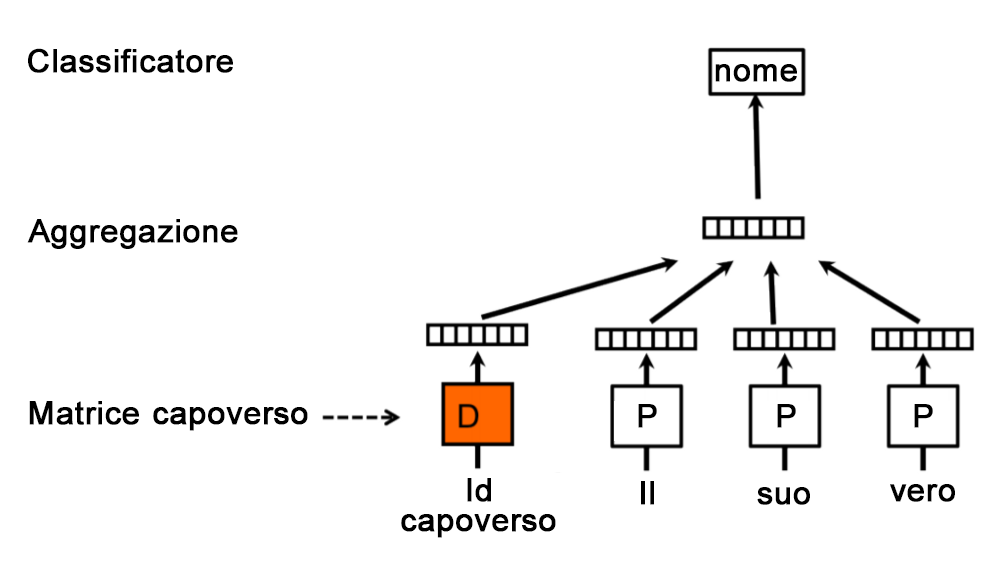
\includegraphics[scale = 0.3]{images/pvdm.png}
    \caption{PV-DM (D sta per documento e P per parola)}
    \label{pvdm}
\end{figure}
\\
La matrice del paragrafo ha gli embedding per i paragrafi "visti", allo stesso modo in cui i modelli Word2Vec apprendono gli embedding per le parole. Per i paragrafi non visualizzati, invece, il modello viene nuovamente eseguito più volte attraverso la discesa del gradiente per inferire un vettore del documento. 

\paragraph{DBOW}
L'architettura DBOW, invece, non utilizza le parole di contesto ma effettua la predizione direttamente dalle parole campionate dal paragrafo.
\\
\begin{figure}[!h]
    \centering
    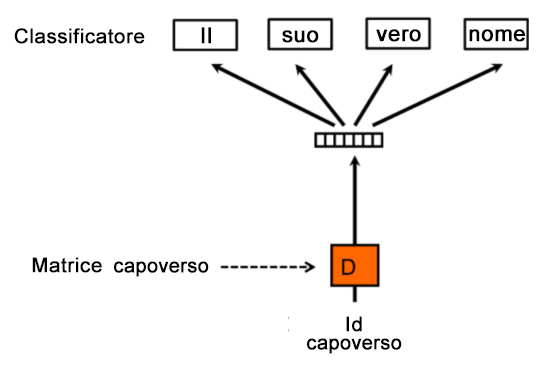
\includegraphics[scale = 0.45]{images/dbow.png}
    \caption{DBOW}
    \label{dbow}
\end{figure}
\\
Ne risulta un'architettura (Figura \ref{dbow}) simile a PV-DM ma con il primo livello costituito unicamente dalla matrice dei paragrafi.

\section{Logica fuzzy} \label{insiemifuzzy}
Dal momento che questo elaborato si pone l'obiettivo di analizzare le notizie e, nello specifico, di valutare un criterio per individuare quelle fake, è importante introdurre il concetto della \textit{logica fuzzy}.
\\
Diversamente da quanto accade per la classificazione, in cui si cerca di associare un valore di verità (vero o falso) per una determinata categoria o classe, nella logica fuzzy si quantifica la componente di una classe assegnando un valore continuo tra 0 e 1.
\\
Tale valore prende diversi nomi, come \textit{grado di verità} o di \textit{funzione di appartenenza}.
\\
In altre parole, la logica fuzzy introduce un valore di verità più granulare rispetto alla tradizionale dicotomia binaria, ottenendo valori che indicano anche se l'espressione sia molto vera, poco vera o mediamente vera.
\\
Per questa ragione la logica fuzzy viene considerata un'estensione della logica booleana.
\\
Più che porsi come alternativa alla classificazione, la logica fuzzy è semplicemente adatta a problemi di natura fuzzy.
\\
Nel campo della sentiment analysis, per esempio, cercare di trovare le emozioni contenute in un testo rientra in questo tipo di problemi; sarebbe limitante, infatti, considerare unicamente se un tweet o un post contenga felicità o meno, oppure se sia vero o falso che ci sia rabbia nelle parole del messaggio di una persona.
\\
Più realisticamente, esistono componenti più o meno forti di ciascuna di queste emozioni che si mischiano e che formano, complessivamente, un testo.
\\
Tali misture, inoltre, spesso causano dell'incertezza che, di fatto, è la ragione per cui il problema risulta più complesso e, allo stesso tempo, affascinante.
\\
E' stato dimostrato, inoltre, che l'ambiguità è una caratteristica intrinseca del linguaggio umano.
Rimanendo nell'esempio della sentiment analysis, la presenza di testi con emozioni ambigue è oggi oggetto di ricerca.
\\
Allo stesso modo, può essere comodo modellare il problema delle fake news come un problema fuzzy, andando quindi a produrre un punteggio di affidabilità per una notizia;
potenzialmente, tale punteggio rappresenta quanto la notizia sia fake.

\section{Induzione di funzioni di appartenenza a insiemi fuzzy} \label{induzione}
In letteratura è stato proposto un algoritmo \cite{1} che fa utilizzo di una procedura originariamente nata come tecnica di support vector clustering \cite{23} per poter indurre il grado di appartenenza dei punti a un certo insieme.
\\
I punti fondamentali di questo approccio riguardano determinare la forma dell'insieme fuzzy e inferire i parametri della sua funzione di appartenenza.
\\
Tra le diverse varianti dell'approccio proposto da questo lavoro, una è in grado di lavorare su dati i cui valori di appartenenza non sono esplicitamente disponibili.
\\
Questo si rivela particolarmente utile quando il dataset che si ha a disposizione contenga informazioni relative alla categoria o classe alla quale i punti appartengono.
\\
Ciò che l'algoritmo fa è fissare ogni classe, e applicare su di essa il processo di apprendimento andando a ricavare il valore di appartenenza a tale categoria.

\subsection{Funzione di appartenenza} \label{membership}
Il concetto di funzione di appartenenza si colloca nella teoria degli insiemi e corrisponde alla funzione caratteristica di un insieme.
\\
Fissando l'insieme $A$, la sua funzione di appartenenza è definita come:
\begin{center}
    $\mu_A(x)= \begin{cases} 1 & \mbox{se } x \in A \\ 0 & \mbox{altrimenti} \end{cases}$
\end{center}

Secondo la logica classica, infatti, un insieme è definito come qualunque aggregato (o collezione) di oggetti per il quale sia sempre possibile decidere se un generico oggetto appartiene oppure no all'aggregato stesso.
\\
Quando la funzione di appartenenza è booleana, perchè si basa su due soli possibili valori di verità, si parla di insieme \textit{crisp}.
\\
Nell'ambito delle notizie, questo corrisponderebbe a fissare l'insieme delle fake news, definire una soglia di qualche tipo e classificare ogni notizia come completamente fake o no, a seconda del fatto che appartenga all'insieme.
\\
Lo scopo di questo lavoro, invece, è di rappresentare lo stesso concetto ma in maniera sfumata, producendo informazioni su \textit{quanto} una notizia sia falsa.
\\
Tale rappresentazione ha il vantaggio di poter indicare se una notizia sia più o meno fake di un'altra.
\\
Per questa ragione si introduce il concetto di \textit{grado di appartenenza}, sull'idea di base che il confine di oggetti appartenenti o non appartenenti all'insieme non sia così ben definito.
\\
La funzione di appartenenza, a questo punto, diventa 
\begin{center}
    $\mu_A: X \rightarrow [0,1]$
\end{center}

si tratta di una funzione che associa ad ogni elemento $x$, assunto dalla variabile $X$, un numero reale compreso tra 0 e 1.
\begin{itemize}
    \item se $\mu_A(x) = 1$ allora $x$ appartiene all'insieme $A$
    \item se $\mu_A(x) = 0$ allora $x$ non appartiene all'insieme $A$
    \item se $0 \leq \mu_A(x) \leq 1$ allora $x$ appartiene parzialmente ad $A$ con grado espresso da $\mu_A(x)$
\end{itemize}
Come anticipato nella Sezione \ref{insiemifuzzy}, si tratta di una logica adatta a problemi strutturati in questa maniera.
\\
Esempi di concetti fuzzy sono \textit{giovane}, \textit{ricco}, \textit{alto}, mentre non lo sono \textit{fratello}, \textit{studente}, \textit{professore}.
\\
Per determinare il valore di $\mu_A$ vengono definiti diversi tipi di funzioni di appartenenza: funzione sigma, funzione triangolare, trapezoidale, S-Shape, e altre ancora (Figura \ref{membership_functions}). 
\\
\begin{figure}[!h]
    \centering
    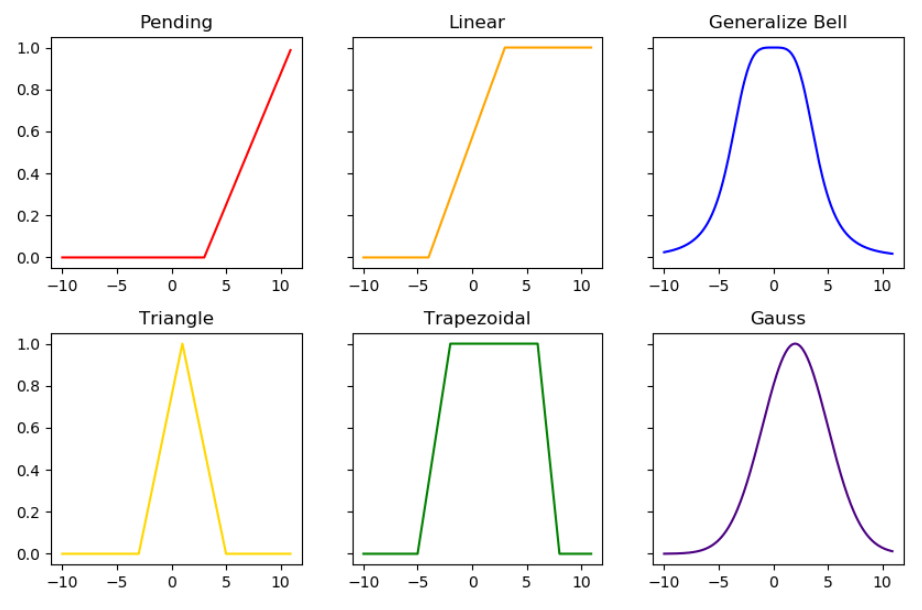
\includegraphics[scale = 0.7]{images/membership_functions.png}
    \caption{Tipi di funzioni di appartenenza}
    \label{membership_functions}
\end{figure}
\\

\subsection{Kernel} \label{kernel}
Si tratta di un oggetto matematico ampiamente utilizzato che, in questo caso, consente di sfruttare le support vector machine anche per problemi di classificazione non lineare.
\\
Questa metodologia prende il nome di \textit{kernel trick} e consiste nel mappare i punti dallo spazio originale a uno spazio a dimensionalità superiore o infinita, dove il problema diventa lineare.
\\
Lo scopo delle SVM, infatti, è quello di trovare l'iperpiano che massimizza il margine dai punti, ma esso esiste se e solo se l'insieme dei punti è linearmente separabile.
\\
Il metodo kernel, quindi, sfruttando le proprietà degli spazi ad alta dimensionalità, permette di applicare le SVM anche per insiemi che non sono linearmente separabili.
\\
Tale vantaggio viene sfruttato per applicare effettivamente il support vector clustering, un tipo di clusterizzazione basato su SVM.
\\
All'interno dello spazio indotto dal kernel si cerca la sfera più piccola che racchiude l'immagine dei punti dello spazio originale.
\\
Questa sfera viene poi rimappata nello spazio originale, dove forma un insieme di contorni che racchiudono i punti; così facendo, i contorni delineano effettivamente il cluster.
\\
Esistono diversi tipi di kernel, ad esempio lineare, polinomiale, iperbolico, gaussiano e molti altri ancora; il tipo di kernel va a impattare sulla forma dei contorni del cluster, in Figura \ref{gaussian} vengono mostrati quattro esempi di clusterizzazione tramite kernel gaussiano con valore crescente del suo iperparametro.
\\
\begin{figure}[!h]
    \centering
    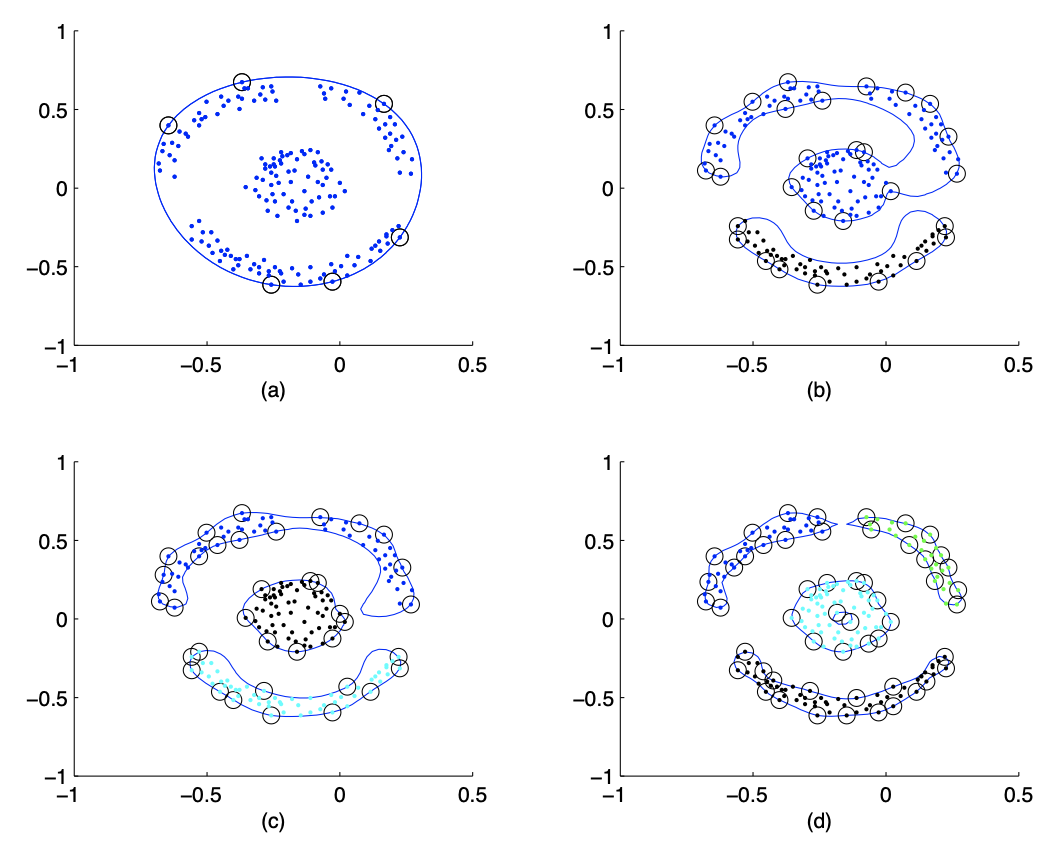
\includegraphics[scale = 0.7]{images/gaussian_kernel.png}
    \caption{Esempi di clusterizzazione con kernel gaussiano - da \cite{23}}
    \label{gaussian}
\end{figure}
\\
La fase successiva è di indurre il valore della funzione di appartenenza a tale insieme.

\subsection{Fuzzificatore} \label{fuzzificatore}
In letteratura i termini \textit{fuzzificazione} e \textit{defuzzificazione} indicano rispettivamente il passaggio da una quantità crisp a una quantità fuzzy e viceversa.
\\
Tale passaggio può avvenire in differenti modi, che dipendono dal tipo di fuzzificatore che si utilizza.
\\
In questo senso è presente anche qui un'ampia scelta di soluzioni: tra quelle più diffuse si menzionano fuzzificatori di tipo lineare ed esponenziale.
\\
Nel caso di questi due fuzzificatori, si starebbe stabilendo se il processo di apprendimento sia fatto facendo decrescere linearmente o esponenzialmente i valori della funzione di appartenenza da 1 a 0.
\\
Geometricamente, questo equivale a definire una certa misura di distanza nello spazio in cui i punti vengono clusterizzati; con grado di appartenenza maggiore essi saranno agglomerati più densamente nel cluster, dualmente con grado minore, i suddetti punti saranno più distanti dall'insieme.

\chapter{Soluzione proposta}
\label{Capitolo 2}
\onehalfspacing
Il secondo Capitolo presenta la soluzione proposta in questo elaborato.
\\
Tale soluzione consiste in un sistema di apprendimento supervisionato a partire dal modello matematico $\bm{\mu}$\textbf{-learn} \cite{1}, la cui struttura viene delineata all'interno della Sezione \ref{mulearn}.
\\
Nella Sezione \ref{sistema}, invece, viene mostrata l'architettura del sistema completo e come il suddetto algoritmo sia stato integrato per poter lavorare su dati testuali inerenti a notizie.

\section[\texorpdfstring{Il modello $\mu$-learn}%
                        {mu-learn}]% % choose text-only material here
        {Il modello $\bm{\mu}$-learn}  % note use of \bm ("bold math")
\label{mulearn}
Si tratta di un algoritmo che utilizza una procedura originariamente nata nel contesto del support vector clustering.
\\
Essa si colloca nel gruppo di tecniche che lavora su insiemi fuzzy triangolari, trattando un problema di ottimizzazione non lineare.
\\
La natura di questo problema si rivela conveniente per la diversificazione delle funzioni di appartenenza, i cui parametri vanno a determinare la forma degli insiemi fuzzy formati.
\\
Il nome di questo modello suggerisce il suo obiettivo: apprendere $\mu$, il grado di appartenenza a un determinato insieme fuzzy.

\subsection{Support vector clustering modificato}
L'assunzione di partenza è disporre di un dataset di punti, ciascuno associato a un proprio grado di appartenenza $\mu$ a un insieme fuzzy sconosciuto.
\\
L'obiettivo è individuare tale insieme e determinare $\mu$ relativamente ad ogni punto.
\\
Il modello ricorre, quindi, alla tecnica di support vector clustering \cite{23} per raggruppare agglomerati di punti in uno spazio in cui essi sono mappati tramite il kernel trick.
\\
Successivamente, verifica se l'immagine $\mathit{\Phi}$ dei punti appartenga a una sfera di raggio $R$ e centro $a$ inizialmente sconosciuti e, infine, determina il grado di appartenenza sulla base della distanza tra esse e il centro.
\\
Il problema di ottimizzazione non lineare a cui si accennava in precedenza riguarda, quindi, la minimizzazione della sfera che racchiude l'immagine dei punti mappati in questo spazio.
\\
I punti racchiusi, infatti, faranno parte dell'insieme fuzzy individuato.
\\
Quelli che seguono sono i tre vincoli del problema
\begin{equation}\label{vincolo}
    \mu_i || \mathit{\Phi}(x_i) - a ||^2 \leq \mu_iR^2 + \xi_i \;,
\end{equation}
\begin{equation}\label{vincolo_2}
    (1 - \mu_i) || \mathit{\Phi}(x_i) - a ||^2 \geq (1 - \mu_i)R^2 + \tau_i \;,
\end{equation}
\begin{equation}\label{vincolo_3}
    \xi_i \geq 0, \tau_i \geq 0 \;.
\end{equation}
la soluzione originale viene, quindi, estesa minimizzando $R^2 + C\sum(\xi_i + \tau_i)$ tramite (\ref{vincolo}-\ref{vincolo_3}), dove $C$ è un iperparametro.

\subsection{Induzione di insiemi fuzzy}
L'ultima fase di induzione della funzione di appartenenza dipende dalla scelta di $C$.
\\
Per questa ragione è necessario uno step di \textit{model selection} in cui si fa tuning dei valori possibili per andare a cercare quelli che meglio si adattano al tipo di dato che si ha a disposizione.
\\
Naturalmente, tale selezione avviene tenendo conto di tutti quei criteri che cercano di prevenire problemi di overfitting e underfitting.
\\
Tipicamente, questo avviene facendo una grid search di un certo intervallo di valori, al fine di valutare il loro impatto con quanti più training e test set possibili, mantenendo coerente la rappresentatività della popolazione.

\subsection{Iperparametri}
Per quanto concerne l'algoritmo sopracitato, ci sono due principali attori: il parametro del kernel e $C$.
\\
Il primo dipende strettamente dal tipo di kernel che si utilizza e condiziona la forma dell'insieme indotto, si pensi ad esempio a $\sigma$ per il kernel gaussiano.
\\
Il secondo impatta sulla dimensione del cosiddetto \textit{core} dell'insieme: più il valore si avvicina all'unità più i punti membri si rivelano essere quelli con grado di appartenenza diverso da zero.
\\
In quanto iperparametri, essi determinano i gradi di libertà del modello che si vuole ottenere.
\\
A tal proposito, è importante avere un campione sufficientemente grande per poter compensare la differenza tra bias e variance error.
\\
Come è ben noto in letteratura, infatti, tale differenza causa dualmente problemi di overfitting e underfitting al prevalere dell'uno sull'altro.
\\
Inoltre, il valore di questi iperparametri deve essere scelto con cura in quanto gioca un ruolo chiave per l'ottenimento di risultati positivi e affidabili; pertanto, a maggior ragione la fase di model selection è importante che venga fatta con attenzione.

\section{Il sistema}
\label{sistema}
Nella presente Sezione si mostra ad alto livello l'architettura della soluzione proposta in questo elaborato, mostrando poi come sia stato utilizzato il modello $\mu$-learn nel contesto del riconoscimento delle fake news.
\subsection{Architettura}
\subsection{Utilizzo dell'algoritmo}

\chapter{Implementazione}
\label{Capitolo 3}
\onehalfspacing

\section{Pipeline di preprocessing}
\subsection{Lowercasing e rimozione del rumore}
\subsection{Lemmatizzazione}
\subsection{Rimozione delle stop word}
\subsection{Word2Vec}
\subsection{Aggregazione}
\section{Selezione dei modelli}
\subsection{Tuning degli iperparametri}
\subsection{Cross validation}
\subsection{Grid search}
\section{Valutazione dei modelli}
\subsection{Matrice di confusione}
\subsection{Precision, Recall e F1}

\chapter{Valutazione sperimentale}
\label{Capitolo 4}
\onehalfspacing
\section{Dataset}
\subsection{Dataset Kaggle}
\subsection{Campione}
\subsubsection{Estrazione del campione}
\section{Esperimenti}
\subsection{Analisi descrittiva}
\subsection{Curve di livello}
\subsection{Performances dei modelli}
\subsection{Baseline}
\subsection{Confronto dei modelli vs baseline}
\section{Vantaggi dell'approccio proposto}
\subsection{Classe di indecisione}
\subsection{Modello LDA}
\subsection{Approssimazione delle membership}

\chapter*{Conclusioni e sviluppi futuri}
\addcontentsline{toc}{chapter}{Conclusioni e sviluppi futuri}
\markboth{Conclusioni e sviluppi futuri}{} 
\onehalfspacing

Integrare l'analisi delle fake news con tecniche di image e video processing per modellare il problema più complesso in cui anche immagini e video svolgono un ruolo centrale nelle fake news (es: immagini vecchie riusate per notizie nuove, video che non corrispondono ai fatti riportati).

\printbibliography

%			RINGRAZIAMENTI
%
\prefacesection{Ringraziamenti}

\end{document}



